En 1931, Kappler proposa une expérience permettant d'observer l'effet des fluctuations thermiques et de déterminer la valeur de la constante de Boltzmann. Un petit miroir plan est suspendu au bout d'un fil possédant une constante de torsion $K$. L'ensemble est placé dans une enceinte contenant un gaz maintenu à la température $T$ (voir la figure \ref{FigKappler}). En mesurant la déviation d'un faisceau lumineux se réfléchissant sur le miroir, on enregistre les fluctuations au cours du temps de $\theta$, l'angle de rotation du miroir par rapport à sa position d'équilibre. L'énergie du miroir est
$$
H(\theta, p_{\theta})=\frac{p_{\theta}^2}{2 \cal I}+
\frac{1}{2}K\theta^2 \enspace,
$$
où $p_{\theta}$ est l'impulsion généralisée associée à la rotation angulaire et $\cal I$ le moment d'inertie du miroir.


\begin{figure}[h]
\begin{center}\scalebox{0.4}{
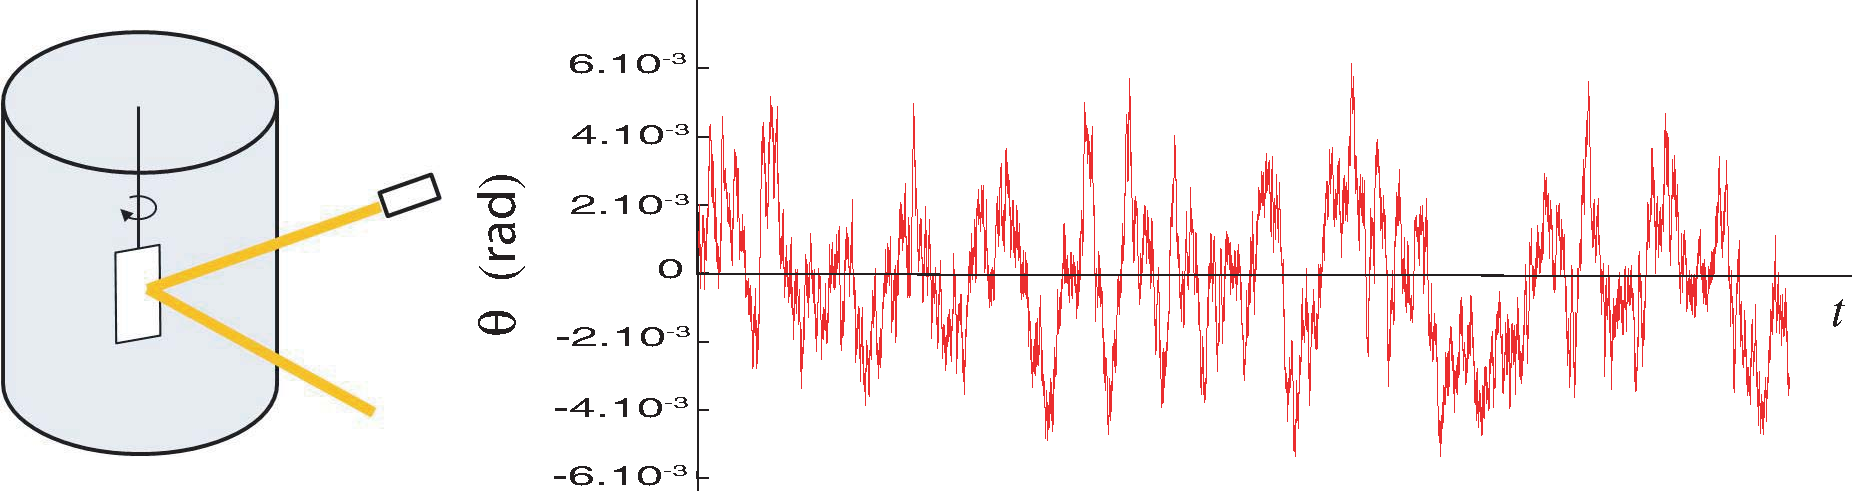
\includegraphics{../Fig/kappler}}
\caption{\it \`A gauche : schéma de l'expérience de Kappler. \`A
  droite : exemple de courbe $\theta(t)$ obtenue en enregistrant la
  déviation du faisceau lumineux au cours du temps.\label{FigKappler}}
\end{center}
\end{figure}


\question
Pour quelle raison le miroir effectue-t-il de petites oscillations autour de sa position d'équilibre ? 

\question
\'Ecrire la distribution de probabilité $P(\theta)$ de l'angle de rotation.  Calculer $\langle {\theta} \rangle$ et Var$(\theta)$.

\question
\`A partir de la courbe $\theta(t)$ reportée sur la figure \ref{FigKappler}, estimer l'écart type de $\theta$. La raideur du fil est $K\simeq 10^{-15}$\,J.rad$^{-2}$ et la température $T\simeq 300$ K. En déduire une valeur estimée de la constante de Boltzmann. 
